\chapter{Methods}\label{ch:03methods}
%TODO Remove this chapter description?
With an understanding of the basics from Chapter~\ref{ch:02background}, in this chapter an overview of the contributions of this thesis and an outline of the methods used in the experiments are presented. 

\section{Contributions}
The main contribution of this thesis is a structured examination of the effects of differing conditions towards reductive evolution in simulated bacteria, as well as how these conditions affect the genome structure of these bacteria. By only changing one variable at a time, the effects of each individual condition on these goals may be isolated from the other factors, providing a clearer picture of their individual impacts. With some insights gained into the mechanisms behind reductive evolution, it is hoped that this may be mapped onto real-world organisms such as \textit{Prochlorococcus}. 

\section{Experimental Designs} \label{experimental_design}

To assist in determining which conditions might lead to reductive evolution, one must isolate individual variables and change just one thing at a time in order to see what effect, if any, it has on the final genome. To that end, a series of experiments were designed and conducted in which a ``wild type'' genome was allowed to evolve in differing conditions for 500,000 generations before analyzing the effects. To first create the wild type, a genome was generated randomly in Aevol which had at least one coding gene and which was allowed to evolve for 10 million generations in a non-varying environment. By the beginning of its use in these experiments, the wild type comprised 13,237 base pairs with 132 functional genes (i.e. genes which produce a gene product) and around 37\% non-coding DNA. The wild type was generated by Guillaume Beslon\textemdash a Computer Science professor at the National Institute of Applied Science in Lyon and a developer of the Aevol platform\textemdash and provided for these thesis experiments. 

In these experiments, separate clonal populations of the wild types were created, one for each condition (including one for the controls) using the Aevol command \texttt{aevol\_create}. These populations were then allowed to continue to evolve in a static environment (using the Aevol command \texttt{aevol\_run}) in a total of 6 different conditions: with an increased/decreased selection strength ($k_+$/$k_-$), an increased/decreased mutation rate ($\mu_+$/$\mu_-$), and an increased/decreased population size ($N_+$/$N_-$). 

For all experiments here, the original target environmental function in which the wild types were generated was also used. This environmental target function, $f_E$, is comprised of three Gaussian functions $y_(x)$, each of which is characterized by a height $h$, mean $m$, and width $w$:
\begin{equation*}
y(x) = h * e^{\left(\frac{-(x-m)^2}{2 * w^2} \right)}
\end{equation*}

A visualization of the target function used in the experiments, $f_E$, can be seen below in Figure~\ref{fig:target_function}. Each Gaussian's parameters $h$, $m$, and $w$ are given in the figure. The gray shaded area is the phenotypic target area.  

\begin{figure}[H]
	\centering
	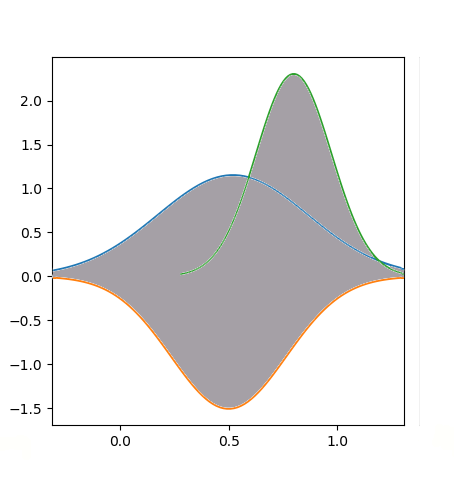
\includegraphics[width=\linewidth]{environmental_target_function01}
	\caption[Experimental target function]{A visual representation of the target function $f_E$ for the experiments.}
	\label{fig:target_function}
\end{figure}

 
In addition to the six tested changed conditions (i.e. $\langle\mu_+$/$\mu_-\rangle$, $\langle k_+$/$k_-\rangle$, and $\langle N_+$/$N_-\rangle$), a control condition experiment was performed in which the wild type was simply allowed to continue to evolve for the 500,000 generations with the same parameters as during the generation of the wild type. To minimize bias, for each condition five runs were performed (that is, 5 rounds of $\mu_+$, 5 rounds of $\mu_-$, etc.), where each run had a differing random seed to control for the deterministic effects of the pseudorandom nature of Aevol's stochastic processes. This lead to a total of 35 experiments, all of which were carried out on a cluster from bwCloud\footnote{\url{https://www.bw-cloud.org/}}. 

The resulting data was processed using a combination of Python\footnote{\url{https://www.python.org/}}, Pandas\footnote{\url{https://pandas.pydata.org/}}, and Jupyter Notebooks\footnote{\url{https://jupyter.org/}}.  

\subsection{Inputs}
In Table~\ref{table:input_parameters}, the parameter values for all input parameters for Aevol may be found. Please note that for $\mu$, this represents the mutation rates for point mutations, small insertions, and small deletions. The rearrangement rates were not changed under any condition and were always $1e-6$ for duplications, deletions, translocations, and inversions. 

\begin{table}[h]
	\centering
	\begin{tabular}{|c||c|c|c|}
		\hline
		 & \multicolumn{3}{c|}{\textbf{Parameter}} \\
		\cline{2-4}
		\textbf{Condition} &$\mu$ & $k$ & $N$ \\
		\hline
		control & $1.00E{-7}$ & $1000$ & $1024$ \\
		\hline
		mutation up ($\mu_+$) & $4.00E{-7}$ & $1000$ & $1024$ \\
		\hline
		mutation down ($\mu_-$) & $2.50E{-8}$ & $1000$ & $1024$ \\
		\hline
		selection up ($k_+$) & $1.00E{-7}$ & $4000$ & $1024$ \\
		\hline
		selection down ($k_-$) & $1.00E{-7}$ & $250$ & $1024$ \\
		\hline
		population up ($N_+$) & $1.00E{-7}$ & $1000$ & $4096$ \\
		\hline
		population down ($N_-$) & $1.00E{-7}$ & $1000$ & $256$ \\		
		\hline
	\end{tabular}
	\caption[Table of parameters]{Table of input parameters. $\mu$ is the mutation rate, $k$ is the selection strength, and $N$ is the population size.}
	\label{table:input_parameters}
\end{table}
As can be seen in Table~\ref{table:input_parameters}, only one parameter varied per condition in order to isolate potential influences on the outcome. A multiplier of $4$ was chosen for the differing conditions relative to the control condition (e.g. $|N_+| = 4096 = 4*|N_\text{control}| = 4*1024$ organisms). This choice of a $4$x multiplier was chosen following the model of Carde et al.\cite{carde.2019}. The goal of their experiments was to use Aevol as a pedagogical tool, teaching a high school student (Carde) to use the scientific method to investigate ``how to reduce a genome.'' The methodology of this thesis is similar to their strategy, namely by providing both an increased and decreased condition for each criteria and otherwise keeping parameters and environments static.


\section{Evaluation Strategy}
In this section, the criteria to be used for evaluating the results are examined. The primary criteria will be calculating the evolved genome's evolvability, robustness, and structure, with a statistical analysis of the changed conditions vs. the control condition. 

\subsection{Statistical Analysis of the Conditions}
First, it must be determined whether the results of the condition (e.g. mutation up, selection down, etc.) were significantly different from the control condition, statistically speaking. To do this, for some test (e.g. robustness, evolvability, etc.) the mean across all seeds is calculated for a condition (e.g. $\mu_+$) and compared to the mean across all seeds of the control condition. For these types of comparison, the ``Mann-Whitney U'' test is used. The Mann-Whitney U test is similar to the Wilcoxon signed-rank test but it is used when the distribution of the two samples cannot be assumed to be normally distributed. The Mann-Whitney U test can also be used when the sample sizes are different, for example when the number of base pairs is different between two organisms.

The purpose of the Mann-Whitney U test is to check whether two independent samples were selected from populations having the same distribution. Similar to other rank-sum tests, the test consists of the following steps:
\begin{enumerate}
	\item Assign numeric ranks to all observations;
	\item Add up the ranks for the observations from the first sample, giving us $R_1$
	\item The statistic $U_1$ for the first sample is given by:
	\begin{equation*}
	U_1 = R_1 - \frac{n_1*(n_1 + 1)}{2}
	\end{equation*}
	where $n_1$ is the sample size for the first sample and $R_1$ is the sum of the ranks from the first sample.
\end{enumerate}
The $U$ statistic for the second sample (i.e. $U_2$) is computed analogously. Then, $U = U_1 + U_2$ which, for sample sizes greater than 20, is approximately normally distributed. Then the standard score is given by:
\begin{equation*}
z = \frac{U - m_U}{\sigma_U}
\end{equation*}
where $m_U$ and $\sigma_U$ are the mean and standard deviation of $U$.
\begin{equation*}
m_U = \frac{n_1*n_2}{2} \text{and } \sigma_U = \sqrt{\frac{n_1*n_2\left(n_1 + n_2 +1\right)}{12}}
\end{equation*} In these experiments, the Python library function \texttt{scipy.stats.mannwhitneyu} was used on Pandas DataFrames containing the observations in order to calculate the Mann-Whitney U statistic. This function also calculates the p-value. With the typical confidence level of $\alpha = 0.05$, if the p-value is below $0.05$, the null hypothesis $H_o$ must be rejected that the two samples (i.e. the control and the condition) are from the same distribution; otherwise it must be accepted.

\subsection{Fitness}
Fitness in Aevol is closely tied in to the ``metabolic error''. This error, $g$, is calculated as the gap between the environmental function $f_E$ and the phenotype of the organism, $f_P$. Once $g$ is determined as described above in Section~\ref{subsec:aevol_selection}, it may be used to calculate the actual fitness of the organism according to the equation:
\begin{equation*}
\text{fitness} = exp(-k*g)
\end{equation*} 
where k is the \textit{selection coefficient} variable set by the user in a parameter file. Aevol provides fitness statistics both for the fittest individual and for the population at large.
\subsection{Robustness}
Aevol calculates statistics for both mutational robustness as well as antirobustness. Robustness in Aevol is calculated similarly to evolvability (see Section~\ref{aevol:evolvability}): a \texttt{lineage} file (see~Section~\ref{sec:aevol_analysis}) for an individual is fed to the post-treatment \texttt{misc\_ancestor\_robustness}, which generates a user-specified large number of offspring whose fitness is then measured. The percentage of these offspring which are neutral (i.e. whose phenotype is not affected by the mutations) is the robustness, and the percentage of positive offspring (i.e. those whose fitness is greater than their parent's) determines the antirobustness.

In these experiments, at the end of the run of 500,000 generations a lineage file for the best individual at generation 500,000, i.e. the individual whose metabolic error was smallest, is generated. This lineage file is then fed in to the post-treatment \texttt{aevol\_misc\_ancestor\_robustness} and robustness statistics are generated for each generation in the lineage file. The statistics produced by this post-treatment are summarized in Table~\ref{table:robustness} below.
\begin{table}[H]
	\centering
	\begin{tabular}{||c||}
		\hline
		\textbf{Statistic} \\
		\hline \hline
		Fraction of positive offspring \\
		\hline
		Fraction of neutral offspring (aka reproductive robustness) \\
		\hline
		Fraction of neutral mutants (aka mutational robustness) \\
		\hline
		Fraction of negative offspring \\
		\hline
		Cumulative delta-gaps of positive offspring \\
		\hline
		Cumulative delta-gaps of negative offspring \\
		\hline
		Delta-gap for the best offspring \\
		\hline
		Delta-gap for the worst offspring \\
		\hline
		Cumulative delta-fitness of positive offspring \\
		\hline
		Cumulative delta-fitness of negative offspring \\
		\hline
		Delta-fitness for the best offspring \\
		\hline
		Delta-fitness for the worst offspring \\
		\hline
		
	\end{tabular}
	\caption[Aevol robustness statistics]{Table of robustness statistics calculated by Aevol for the best individual with the provided lineage.}
	\label{table:robustness}
\end{table}
These statistics for both the control and the specific desired condition (e.g. mutation up) may then be compared. Because this data is somewhat noisy (owing to the fact that the fitness may change rapidly), occasionally box and whisker plots will be used to show the overall spread rather than plotting the robustness generation by generation. 
\subsection{Evolvability}\label{aevol:evolvability}
In Aevol, evolvability is calculated by generating a large set of offspring for a specific individual (one whose lineage was generated using the post-treatment \texttt{aevol\_misc\_lineage}) at regular periods along their lineage and then determining the number of ``positive offspring''. Positive offspring are defined as those whose fitness is greater than their parent's. The evolvability of an individual is then the sum total of all improvement of all of the beneficial offspring, i.e.:

\begin{equation*}
\text{evolvability} = \frac{|\text{positive offspring of }i|}{|\text{total offspring of }i|}*\sum \Delta^{\text{positive offspring}}_{fitness}
\end{equation*}  where $\sum \Delta^{\text{positive offspring}}_{fitness}$ is the cumulative sum of the fitness increase for the positive offspring. Thus, evolvability in Aevol accounts for both the likelihood of a positive mutation and the average improvement provided by said mutation. Practically speaking, to find an organisms evolvability in Aevol one must give the post-treatment \texttt{misc\_ancestor\_robustness} a lineage file and then multiply the fraction of the number of positive offspring (column 2) by the cumulative total of the fitness gap $g$ of the positive offspring (column 10).

%\subsubsection{Time to Coalescence}

 
\subsection{Structure}\label{methods:structure}
Another strength of Aevol is its ability to analyze changes in the structure of DNA and RNA. As with fitness, Aevol produces statistics about individuals and the population at large for many aspects of genome structure, including: the number of coding vs. non-coding bases (i.e. they respectively do or do not code for at least one protein), the average size of coding and non-coding DNAs, the number of genes, the number of ``essential'' base pairs (i.e. those that are part of a functional coding sequence), etc. Tables~\ref{table:aevol_stats_genes_and_bp} and Table~\ref{table:aevol_stats_fitness_and_mutation} summarize the different statistics and where they are to be found Aevol's output files. 

As mentioned in Section~\ref{related_work}, Koskiniemi et al.~\cite{koskiniemi2012} tested the hypothesis that reductive evolution might occur partly as a result of selection, where fitness is gained by selecting for a 

%TODO Flesh out motivation for including non-coding bases as a performance measure
Non-coding bases determine regulation %TODO Find source for this - read it just on Wikipedia
	

\begin{table}[H]
	\centering
	\begin{tabular}{ |c|c| }
		\hline
		\multicolumn{2}{|c|}{\textbf{Stat File}} \\
		\hline
		\texttt{stat\_genes\_}$\langle$\texttt{best/glob}$\rangle$ & \texttt{stat\_bp\_}$\langle$\texttt{best/glob}$\rangle$ \\
		\hline \hline
		number of coding RNAs & number of bp not in any CDS \\
		\hline
		number of non-coding RNAs & number of bp not included in any functional CDS \\
		\hline
		average size of coding RNAs & number of bp not included in any non-functional CDS \\
		\hline
		average size of non-coding RNAs & number of bp not included in any RNA \\
		\hline
		number of functional genes & number of bp not included in any coding RNA \\
		\hline
		number of non-functional genes & number of bp not included in any non-coding RNA \\
		\hline
		average size of functional genes & number of non-essential bp \\
		\hline
		average size of non-functional genes & number of non-essential bp including non-functional genes \\
		\hline
	\end{tabular}
	\caption[Aevol's stats: genes and base pairs]{Statistics found in \texttt{stat\_genes} and \texttt{stat\_bp} output files from Aevol. $\langle$best/glob$\rangle$ indicates that statistics are available for both the best individual and the average across the whole population.}
	\label{table:aevol_stats_genes_and_bp}
\end{table}
``Essential'' base pairs are those whose mutation would change the phenotype of the organism.
\begin{table}[H]
	\centering
	\begin{tabular}{ |c|c| }
		\hline
		\multicolumn{2}{|c|}{\textbf{Stat File}} \\
		\hline
		\textbf{stat\_fitness\_$\langle$best/glob$\rangle$} &
		\textbf{stat\_mutation\_$\langle$best/glob$\rangle$} \\
		\hline \hline
		population size & number of local mutations \\
		fitness & number of chromosomic rearrangements \\
		genome size & number of switches \\
		metabolic error & number of indels \\
		parent's metabolic error & number of duplications \\
		metabolic fitness & number of deletions \\
		secretion error & number of translocations \\
		parent's secretion error & number of inversions \\
		secretion fitness & \\ 
		amount of compound present in grid-cell & \\
		\hline
	\end{tabular}	
	\caption[Aevol's stats: fitness and mutation]{Statistics found in \texttt{stat\_fitness} and \texttt{stat\_mutation} files from Aevol. $\langle$best/glob$\rangle$ indicates that statistics are available for both the best individual and the average across the whole population.}
	\label{table:aevol_stats_fitness_and_mutation}
\end{table}
 
\section{Expected Results}\label{sec:expected_results}
%TODO Expand on this section
Table~\ref{table:experiment_predictions} gives the expected behavior for each of the six conditions investigated in this thesis based on the literature review from Section~\ref{related_work}. A `$+$' indicates that an increase is expected in that area (e.g. genome size) and a `$-$' indicates an expected decrease.
\begin{table}[H]
	\centering
	\begin{tabular}{|c||c|c|c|c|c|c|}
		\hline
		\multicolumn{7}{|c|}{{\Large \textbf{Experiment Predictions}}} \\
		\hline \hline
		\multirow{2}{*}{\textbf{Effect on:}} & \multicolumn{6}{c|}{\textbf{Condition}} \\
		\cline{2-7}
		 & {\Large$\mu_+$} & {\Large$\mu_-$} & {\Large$k_+$} & {\Large$k_-$} & {\Large$N_+$} & {\Large$N_-$} \\
		\hline \hline
		Genome Size & $-^{\cite{bradwell2013correlation,  carde.2019, marais2008mutation}}$ & $\text{+}^{\cite{bradwell2013correlation, carde.2019, drake1991constant}}$ & $+^{\cite{Batut.2013}}$ & $-^{\cite{Batut.2013}}$ & $-^{\cite{Batut.2014, carde.2019}}$ & $+^{\cite{Batut.2014,carde.2019}}$ \\
		\hline
		Fitness & $+^{\cite{bataillon2000estimation, vahdati2017effect}}$ & $-^{\cite{vahdati2017effect}}$ & $+^{\cite{Batut.2014}}$ & $-^{\cite{Batut.2014}}$ & $+^{\cite{cutter2019primer, vahdati2017effect}} $ & $-^{\cite{cutter2019primer, vahdati2017effect}} $\\
		\hline
		Amount of non-coding DNA & $-^{\cite{Knibbe2007}}$ & $+^{\cite{Knibbe2007}}$ & $+^{\cite{Batut.2013, Knibbe2007}}$ & $-^{\cite{Batut.2013, Knibbe2007}}$ & $-^{\cite{Batut.2013}}$ & $+^{\cite{Batut.2013}}$ \\
		\hline
		Number of genes & $-^{\cite{Knibbe2007}}$ & $+^{\cite{Knibbe2007}}$ & $+^{\cite{Knibbe2007}}$ & $-^{\cite{Knibbe2007}}$ & $-^{\cite{Batut.2014}}$ & $+^{\cite{Batut.2014}}$ \\
		\hline
		Average size of genes & $-^{\cite{Liard.2018}}$ & $+^{\cite{Liard.2018}}$ & $-^{\cite{Batut.2013}}$ & $+^{\cite{Batut.2013}}$ & $-^{\cite{Batut.2014}}$ & $+^{\cite{Batut.2014}}$ \\
		\hline
		Robustness & $-^{\cite{Knibbe2007}}$ & $+^{\cite{Knibbe2007}}$ & $-^{\cite{Batut.2013, Knibbe2007}}$ & $+^{\cite{Batut.2013, Knibbe2007}}$ & $-^{\cite{elena2007effects}}$ & $+^{\cite{elena2007effects}}$ \\
		\hline
		Evolvability & $+^{\cite{Knibbe2007}}$ & $-^{\cite{Knibbe2007}}$ &  $+^{\cite{Batut.2013}}$ & $-^{\cite{Batut.2013}}$ & $-^{\cite{wein2019effect}}$ & $+^{\cite{wein2019effect}}$ \\
		\hline		
	\end{tabular}
	\caption[Experiment expectations]{Predictions for the experiments. $\mu$ is the mutation rate, ~$k$ is the selection rate, and $N$ is the population size. $\mu_+$ indicates an increased mutation rate, $\mu_-$ a decreased rate, etc. A $+$ in the main grid space indicates an expected increase (over the control condition) for that condition, and a $-$ indicates an expected decrease for that condition.}
	\label{table:experiment_predictions}
\end{table}
As summarized in the table, a reduction in genome size is expected to occur in the $\mu_+$, $k_-$, and $N_+$ conditions. Based on the work of Bradwell et al., Carde et al., and Marais et al. \cite{bradwell2013correlation, carde.2019, marais2008mutation}, it is expected that an increased mutation rate (i.e. the $\mu_+$ condition) should cause many deleterious mutations which in turn will be removed by purifying selection. Likewise, with weaker selection, the work of Batut et al. \cite{Batut.2013} indicates that with a decreased selection pressure (corresponding to the $k_-$ condition here), many functional genes are lost, causing the organisms to be less fit on average. More interestingly, however, the reduced selection pressure is also expected to cause a loss in non-coding bases, which was the primary source of genome reduction in their experiments. This follows from the fact that, as found in a previous study by Knibbe et al. \cite{Knibbe2007}, the most successful genomes tend to be those that produce ``a little more than one `neutral offspring', that is to say, offspring without mutations or with only neutral mutations'' \cite{Batut.2013}. More formally, Knibbe et al. found that successful genomes fulfill $F_v*W \approxeq 1$, where $W=\frac{e^{-k*g}}{\sum_{i=1}^{N}e^{-k*g}}$ is the expected number of offspring ($k$ is the selection coefficient and $g$ is the gap described in Section~\ref{subsec:aevol_selection}) and $F_v$ is the probability of an offspring having either no mutations or only neutral ones. In other words, with reduced selection, $F_v$ is increased because non-coding DNA is mutagenic for the surrounding genes, so a certain level of mutational variability is still selected for. Lastly, based on the work in another publication by Batut et al. \cite{Batut.2014}, an increase in population size (corresponding to the $N_+$ condition) is expected to cause a decrease in genome size, most likely because of the increased efficacy of selection in larger populations. 

Robustness \& Evolvability
1) Robustness mirrors genome size except in the case of selection
2) Evolvability mirrors genome size except for population size



